% !TEX TS-program = xelatex
% !TEX encoding = UTF-8 Unicode
% !Mode:: "TeX:UTF-8"

\documentclass{resume}
\usepackage{zh_CN-Adobefonts_external} % Simplified Chinese Support using external fonts (./fonts/zh_CN-Adobe/)
%\usepackage{NotoSansSC_external}
%\usepackage{NotoSerifCJKsc_external} \usepackage{zh_CN-Adobefonts_internal} % Simplified Chinese Support using system fonts
\usepackage{linespacing_fix} % disable extra space before next section
\usepackage{cite}
\usepackage{graphicx}
\usepackage{tabu}
\usepackage{multirow}
\usepackage{progressbar}

\begin{document}
	
\pagenumbering{gobble} % suppress displaying page number

\begin{center}
	\Large
\begin{tabu}{ c l r }
		\multirow{5}{1in}{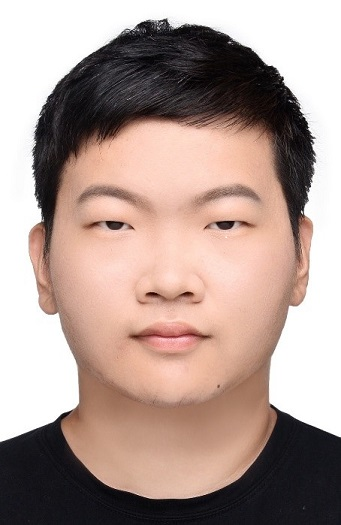
\includegraphics[width=0.12\textwidth]{cd2}} & \scshape{常迪} & {Python~}\progressbar{0.9} \\
		& \email{2862588711cd@gmail.com} & {Matlab}\progressbar{0.9} \\
		& \phone{(+86) 188-428-32169} & {Latex}\progressbar{0.8} \\
		& \linkedin[Chang Di]{https://www.linkedin.com/in/chang-di-004784206} & {C}\progressbar{0.6} \\
		& \github[Boese0601]{https://github.com/Boese0601} & {Javascript}\progressbar{0.6}
\end{tabu}
\end{center}



\basicInfo{}
 
\section{\faGraduationCap\  教育背景}
\datedsubsection{\textbf{大连理工大学}, 大连,辽宁}{2018.9 -- 至今}
\textit{在读本科生}\ 电子信息工程, 预计 2022 年 9 月毕业
\begin{itemize}
	\item 总GPA : 91.1/100 \quad 3.91/4.0 \qquad|| \qquad 专业课GPA : 93.0/100\quad 3.95/4.0 
	\item 院系排名 : 10/210  \qquad   前5 \%
	\item 部分课程 : 数学分析:100\quad 计算机组成原理:96 \quad 数字电路与系统:96 \quad 离散数学:98 \\概率论与数理统计:98 \quad 数据结构与算法:93
\end{itemize}
\datedsubsection{\textbf{慕尼黑工业大学}, 慕尼黑, 拜仁州}{2021.10 -- 2022.9}
\textit{本科交换生}\ 计算机科学与工程,已被录取,预计2021年10月派出
\datedsubsection{\textbf{帝国理工学院}, 伦敦}{2021.1 -- 2021.3}
\textit{寒假学校}\ 数据科学与计算机视觉
%\datedsubsection{\textbf{加州大学圣地亚哥分校}, 圣地亚哥,加利福尼亚}{2019.6 -- 2019.8}
%\textit{暑期学校}\ 电子与计算机工程

\section{\faUsers\ 实习/科研/项目经历}
\datedsubsection{\textbf{图像智能分析与理解实验室(IIAU-Lab)}\quad 信息与通信工程学院}{2020年1月 -- 至今}
\role{科研助理}{指导教师:卢湖川(国家杰出青年基金获得者,创新与创业学院院长,人工智能学院副院长)}
\textit{目前的方向主要集中在如何改进现有的多阶段目标检测算法与单/多目标跟踪算法,并对语义分割算法进行了解与实际应用。阅读导师推荐的关于分割、检测、追踪的论文,并在每周小组会议上做出对近期提出的新论文中的算法的汇报。
	应用已经成熟的目标检测算法并作出改进参加Kaggle或和鲸社区等其他单位组织的比赛,取得了较好的名次和成绩,并通过复现实验室自行提出的算法并将其用于实际的工业场景来评测算法的应用价值与实用度。
}

\datedsubsection{\textbf{IIAU 项目1:2020全国水下机器人目标检测算法赛}}{2020.3 -- 2020.12}
\role{队长}{团队项目,与组内另一位本科生共同开发\qquad 指导教师:王栋(IIAU-Lab副教授)}
\begin{onehalfspacing}
COCO数据集,赛道为水下生物四分类光学图像目标检测\\https://github.com/Boese0601/2020-Underwater-Detection-Final
\begin{itemize}
  \item 使用Cascade-RCNN+ResNext101+FPN作为基本框架
  \item 应用mosaic,RandomRotate90°等数据增强技术减少网络过拟合改进模型
  泛化能力
  \item 利用多尺度训练和预测来适应图像分辨率的差异,使得目标的大小不同
  训练中所涉及的分布更加均衡,使得模型对目标尺寸具有更好的鲁棒性
  \item 应用soft-nms以及Cutout以提高岩石覆盖或重叠目标的检测率
  \item 使用可变形卷积DCN代替普通CNN操作,增加了很少的模型复杂度和计算量,但显著提高了识别精度
\end{itemize}
成绩:B榜Map49.69 排名:6/210
\end{onehalfspacing}

\datedsubsection{\textbf{IIAU 项目2:无人机视觉:行人与车辆检测与跟踪}}{2020.12 -- 至今}
\role{组内成员}{实验室项目,组内硕士博士为主要算法开发成员}
\begin{onehalfspacing}
目标:实现无人机跟随目标车辆飞行并且对行人及其他路面情况进行应急反应与处理
\begin{itemize}
  \item 平台: NVIDIA Jetson Xavier NX/NVIDIA Jetson TX2
  \item 算法框架: YoloV5检测算法+JDE多目标跟踪算法(CVPR 2020)
  \item 第一步:输出物体中心点的xy坐标。数据稳定,无大波动,无异常框架。无人机将当前的欧拉角数据发送给视觉模块。\\
  第二步:视觉模块将计算出的高度数据和欧拉角相结合,然后将XY方向的距离误差发送给无人机。\\
  第三步:无人机提供欧拉角信息,视觉模块作为控制中心,直接发送四轴的期望速度数据。
\end{itemize}
\textit{注:此项目仍在进行中,代码不方便开源,如有需求请直接与我沟通}
\end{onehalfspacing}\\
\datedsubsection{\textbf{校外项目1:医学图像分类与语义分割}\quad 数据科学学院,帝国理工学院}{2021.1--2021.3}
\role{小组组长}{指导教师:Dr.Chengliang Dai(帝国理工学院助理教授,研究员)}
\textit{开发一种可靠的新型脑瘤分类与语义分割模型从给出的医学影像数据集中检测出胶质瘤}\\
https://github.com/Boese0601/ImperialCollegeLondon\_DSI\_Winter
\begin{itemize}
	\item 分类任务:VGG19 + 特定医学图像增强方法,验证集准确度0.9516
	\item 分割任务:ResNet152 backbone + U-Net+++(CVPR 2020)验证集Dice\_score 0.9025
	\item 复现了多篇医学领域的增强方法,入手角度包括SeGAN,cGAN等生成图像,传统的翻转、镜像、亮度调节、伸缩放缩的方法,尝试了Deep Supervision等方法
\end{itemize}
最终结项答辩成绩:1/95\\
\datedsubsection{\textbf{实习1:网络前端见习工程师}}{2020.6 -- 2020.8}
\role{实习生} {大连豪森瑞德-豪森智源数据有限公司,技术部}
\textit{为公司网页提供表单设计及其他页面制作,并配合后端接口做出调整}
\begin{itemize}
	\item 前端网页与公司的数据库系统构建 (框架:React)
	\item 调试代码并负责网站维护
	\item 参与公司新IOS应用程序开发与设计
\end{itemize}

\section{\faCogs\ IT 技能}
% increase linespacing [parsep=0.5ex]
\begin{itemize}[parsep=0.5ex]
  \item 编程语言:Python == Matlab > Latex > Javascript == C
  \item 平台: Linux(Ubuntu,CentOS),Windows,MacOS
  \item 框架: Keras(TensorFlow),PyTorch,Jittor
\end{itemize}

\section{\faHeartO\ 获奖情况}
\datedline{全国中学生奥林匹克物理竞赛辽宁赛区,\textit{省一等奖,第18名}}{2017年}
\datedline{一等奖学金,\textit{院系前5\%}}{2019年}
\datedline{国家奖学金}{2019年}
\datedline{一等奖学金,\textit{院系前5\%}}{2020年}
\datedline{全国大学生数学建模竞赛,\textit{二等奖}}{2020年}
\datedline{大连理工大学AI挑战赛,目标检测赛道,\textit{全校第二名}}{2020年}
% \datedline{美国大学生数学建模竞赛ICM/MCM,\textit{M奖}}{2021年}

\section{\faInfo\ 语言能力}
% increase linespacing [parsep=0.5ex]
\begin{itemize}[parsep=0.5ex]
  \item 英语 -- C1: IELTS雅思学术类 7.0 (8.0/7.0/6.5/6.0)\qquad GRE 319 (V149+Q170)
  \item 德语 -- B2: TestDaf德福 14/20 (4/4/3/3)
\end{itemize}

\end{document}
